% This file demonstrates how to use the IEEEConf LaTeX2e macro package,
% to prepare a manuscript for proceedings on CD of the conference
% FedCSIS
%
\documentclass[conference]{IEEEtran}
%\documentclass[a4paper]{IEEEconf}

% This package serves to balance the column lengths on the last page of the document.
% please, insert \balance command in the left column of the last page
\usepackage{balance}

%% to enable \thank command
\IEEEoverridecommandlockouts 
%% The usage of the following packages is recommended
%% to insert graphics
\usepackage[dvips]{graphicx}
% to typeset algorithms
% to typeset code fragments
\usepackage{listings}
% provides various features to facilitate writing math formulas and to improve the typographical quality of their output.
\usepackage[cmex10]{amsmath}
\interdisplaylinepenalty=2500
% por urls typesetting and breaking
\usepackage{url}
% for vertical merging table cells
\usepackage{multirow}

% define environments for remarks and examples
\newtheorem{remark}{Remark}[section]
\newtheorem{example}[remark]{Example}


%
%
\title{Czech parliament meeting recordings as ASR training data}
%
%
\author{
\IEEEauthorblockN{Jan Oldřich Krůza}
\IEEEauthorblockA{
Institute of Formal and Applied Linguistics,\\
Faculty of Mathematics and Physics,\\
Charles University\\
Email: kruza@ufal.mff.cuni.cz}
}

% conference papers do not typically use \thanks and this command
% is locked out in conference mode. If really needed, such as for
% the acknowledgment of grants, issue a \IEEEoverridecommandlockouts
% after \documentclass

% for over three affiliations, or if they all won't fit within the width
% of the page, use this alternative format:
% 
%\author{\IEEEauthorblockN{Michael Shell\IEEEauthorrefmark{1},
%Homer Simpson\IEEEauthorrefmark{2},
%James Kirk\IEEEauthorrefmark{3}, 
%Montgomery Scott\IEEEauthorrefmark{3} and
%Eldon Tyrell\IEEEauthorrefmark{4}}
%\IEEEauthorblockA{\IEEEauthorrefmark{1}School of Electrical and Computer Engineering\\
%Georgia Institute of Technology,
%Atlanta, Georgia 30332--0250\\ Email: see http://www.michaelshell.org/contact.html}
%\IEEEauthorblockA{\IEEEauthorrefmark{2}Twentieth Century Fox, Springfield, USA\\
%Email: homer@thesimpsons.com}
%\IEEEauthorblockA{\IEEEauthorrefmark{3}Starfleet Academy, San Francisco, California 96678-2391\\
%Telephone: (800) 555--1212, Fax: (888) 555--1212}
%\IEEEauthorblockA{\IEEEauthorrefmark{4}Tyrell Inc., 123 Replicant Street, Los Angeles, California 90210--4321}}





\begin{document}
\maketitle              % typeset the title of the contribution

\begin{abstract}
I present a way to leverage the stenographed recordings of the Czech parliament
meetings for purposes of training a speech-to-text system. The article presents
a method for scraping the data, acquiring word-level alignment and selecting
reliable parts of the imprecise transcript. Finally, I present an ASR system
trained on these and other data.
\end{abstract}


\section{Introduction}
\label{sec:intro}

Training data for speech recognition is always a demanded commodity, especially
if it is free. There are for sure already some free Czech corpora fit for speech
recognition training:
\begin{itemize}
\item{
    Vystadial\cite{vystadialarticle} with its 77 hours of VoIP
    calls\cite{vystadialdata}, 
}
\item{
    The Prague Database of Spoken Czech\cite{pdtscarticle} with its 122 hours
    of richly annotated spontaneous dialogues\cite{pdtscdata},
}
\item{
    The Czech Senior COMPANION Expressive Speech Corpus with its 5 hours
    of professionally spoken utterances by a single speaker\cite{companiondata},
}
\item{
    Otázky Václava Moravce: 35 hours of transcribed recordings of the
    Czech TV talk show\cite{ovmdata},
}
\item{
    STAZKA, a set of speech recording from vehicles with its 35 hours of
    background noise and utterances\cite{stazkadata},
}
\item{
    Spoken Corpus of Karel Makoň\cite{kruuza2012making} with its 100 hours of
    manually transcribed spontaneous speech by a single speaker\cite{makondata},
}
\item{and possibly others that I am not aware of.}
\end{itemize}

The Czech parliament meeting recordings represent a publicly available dataset
of high-quality audio recordings of contemporary Czech in consistent low-noise
audio quality worth almost 4000 hours of downloadable material, about 2800 hours
after subtraction of the overlaps. Extracting
training data for speech recognition systems would provide a corpus at least
one order greater in length than those so far publicly available.

Verily, I am not the first person to attempt using these recordings for speech
recognition. The Department of Cybernetics of University of West Bohemia
developed an automatic online subtitling system for the meetings in
2006\cite{pspsubs} and as a result, an 88-hour subset annotated by high-quality
automatic transcript has been released for speech recognition training
purposes\cite{pspdata}.

I attempt to use the official stenographic transcripts available for all the
talks so that it can be a new entry in the above list, on par in quality and
excelling in size.

\section{Data Preparation}

Since the source data is publicly available and in the public domain, I merely
provide the scripts for downloading and building the corpus. The algorithms and
parameters used are described in this section.

\subsection{Scraping}

Regrettably, the data are to my best knowledge only available in human-readable
form. The transcript is not clearly distinguished in the markup and is
interlaced with metainformation. My method of isolating the transcript is quite
crude but it covers the vast majority of cases. The criterion is to extract the
subtree of all nodes with HTML attribute \texttt{[align=justify]}, except HTML
elements \texttt{<b>}, which contain speaker identification.

The known shortcomings of this method are that 1) it discards the speaker
annotations, although it is valuable metainformation and 2) it skips some short
passages, e.g. references to other meetings, as can be seen in the meeting
from Feb. 12th 2020 10:10 -
10:20\footnote{https://www.psp.cz/eknih/2017ps/stenprot/040schuz/s040372.htm}.
Both can be corrected by devising a smarter scraper and neither has any
significance for speech recognition: speaker annotation fundamentally and
neglecting the links for their infrequency.

\subsection{Alignment}

One of the obstacles in using the stenographic transcripts for training an ASR
system is the very loose alignment available. The recordings are all 14 minutes
long and have a 4-minute overlap. The corresponding transcript is thus aligned
in 10-minute blocks with a roughly 2-minute padding on each side of the audio.
Figure~\ref{fig:overlap} schematically shows the alignment of the stenographic
transcript to the audio and the overlap of the recordings.

\begin{figure*}[tpb]
\centering
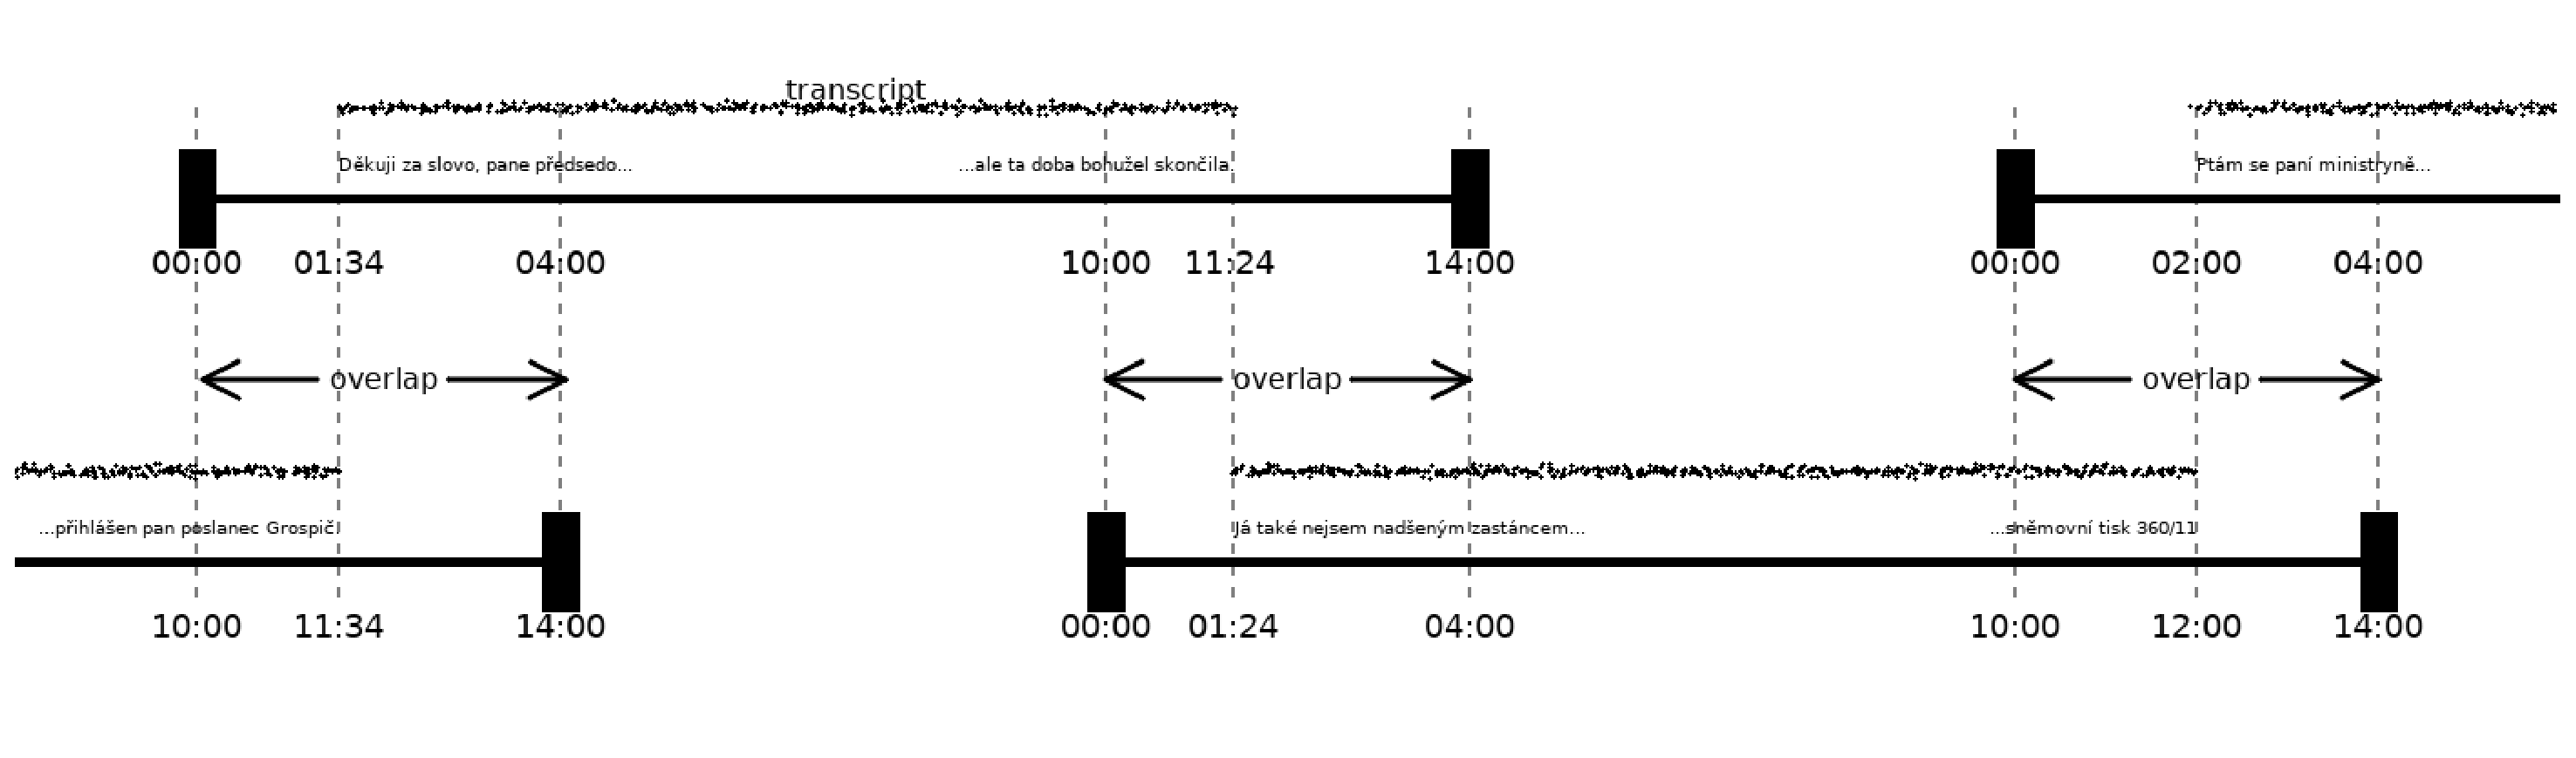
\includegraphics[width=0.9\hsize]{rc/overlap.eps}
\caption{Alignment and overlap of audio files and transcript. The examples are
from Feb. 12th 2020 around 10 o'clock. The transcript corresponding to the
recording in the upper left covers audio positions 01:34 - 11:24. The one in the
lower right from 01:24 to 12:00.}
\label{fig:overlap}
\end{figure*}


Systems for aligning long audio segments to their transcripts already exist,
like that of Moreno et al.\cite{moreno1998recursive} or
Hazen\cite{hazen2006automatic}. They are both based on an already existing
automatically acquired transcript. I use this technique as well, though 
simplified and adapted to the task.

I have used the dataset mentioned above\cite{pspdata} to train a GMM-based ASR
system, using the stenographs as training data for a language model. Using these
models, a word-level-aligned transcript of the whole set of recordings has been
acquired.

The predicted transcript and the stenographic one have then been compared for
Levenshtein distance, determining the edit operations needed to transform one
into the other. For each predicted word, a reliability score is then
computed as 1 - unreliability where unreliability is the number of edit
operations taken on it divided by its length.
Figure~\ref{fig:align} shows how the stenographic transcript is aligned with the
audio on word level.

\begin{figure*}[htpb]
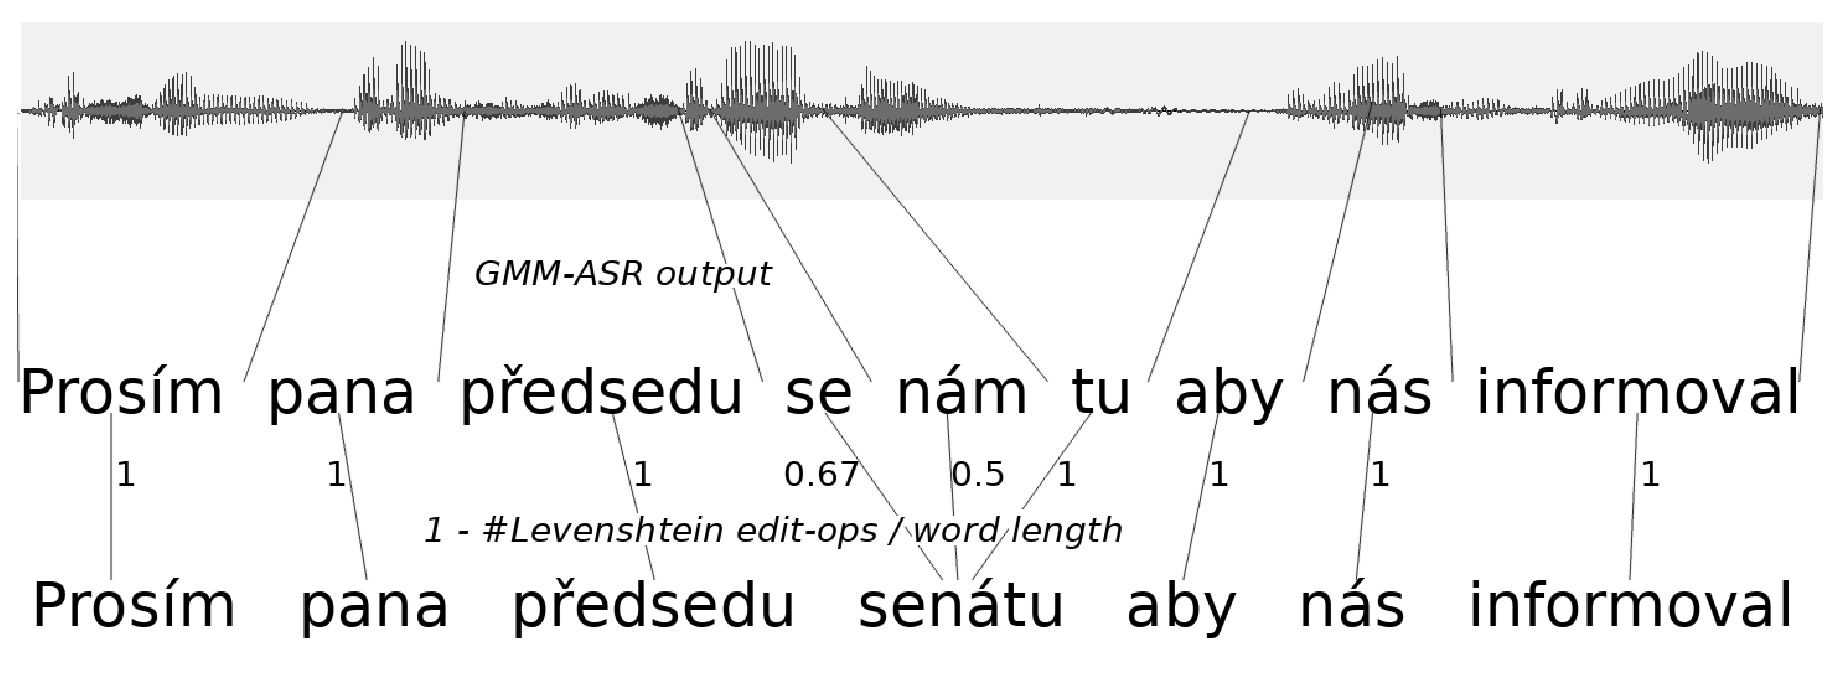
\includegraphics[width=0.9\hsize]{rc/align.eps}
\caption{Schema of aligning the audio to the stenographic transcript on word
level.}
\label{fig:align}
\end{figure*}

Nota bene, a GMM-based system was chosen for the initial transcript instead of
a DNN-based for three reasons: 1) Foremost, it is straightforward to obtain
precise alignment from a GMM-based system. 2) The training doesn't require so
much computational resources and data. 3) It isn't crucial to have maximum possible
accuracy in this stage.

\subsection{Audio Segmentation}

To create a usable dataset for training a speech-to-text system, it is not
necessary to perfectly align the whole transcript. On the contrary, it is
desirable to align what is reliably precise and discard the rest.

The criteria for good training samples are:
\begin{enumerate}
\item{100\% precise transcript,}
\item{roughly sentence-level length,}
\item{consistent length.}
\end{enumerate}

To ensure precise transcript, it is good to have the samples padded by some
silence, since the alignment obtained from the initial ASR may be a bit
imprecise. We thus want to split at pauses, the longer the better, up to a
certain limit (about 1 second). The need to split at longer
pauses goes against the need to split at consistent, none-too-great lengths.

So the problem is to select an optimal set of silences so that the longest ones
are used and so that they split the recording into chunks of length in a given
range. This looks like a problem for dynamic programming but a simpler approach
is also possible: Start with a set of all silences predicted by the forced
alignment.  Iterate over the silences shortest-first and remove each if it
doesn't break the constraints.

I have experimentally set the length boundaries to 12 - 30 seconds. The maximum
length could be decreased at the cost of available pauses to choose from, which
would lead to more frequent splits in the middle of a word.

\subsection{Training Samples Selection}

With the audio segmented and corresponding manual transcripts extracted, the
last step remaining is selecting which segments to include in the traning data.
Indeed, since the recordings have a 2-minute padding on each side for 10 middle
minutes, we must discard at the very least 40\% of the segments. I use the
following criteria for including a segment in the data:

\begin{enumerate}
\item{The first and last token have reliability at least 70\%,}
\item{The mean reliability of all tokens is at least 70\%,}
\item{The number of words is no less than five.}
\end{enumerate}

Minimum reliability of border tokens is considered to minimize the danger of
shifted alignment boundaries. Mean reliability is considered because it is OK
for some words to have very low reliability: there are enough errors in the
prediction, that's why we use the manual transcript after all. But if too many
tokens have too low reliability, then it is a sign of a suspicious segment. The
number of words has a minimum because with only a few words, the probability of
misalignment with good score is much greater than when there are enough words.

Why use mean reliability and not median? The way the reliability is computed
considers the number of edit operations on one line in the automatic transcript.
In the case where there are many insertions, the reliability of one line can go
arbitrarily deep sub zero. So it can happen that there are several inserted
words in a (mis)aligned chunk that only affect the reliability score of a single
word. The mean taps these while the median doesn't.

\subsection{Data Extraction Summary}

All the constants and criteria are to be considered a baseline solution. They
all could be tweaked much more rigorously and solved much more soundly. However,
this simple solution readily yields a high-quality training dataset of 1058
hours. Of the total 539,057 segments, 142,530 (26\%) have been accepted to the
training dataset. Of the total 396,527 discarded segments, 350,258 (88\%) were
discarded because of the criterion of unreliable start or end. It should be
noted however, that the start / end reliability criterion is applied first, so
it catches segments that would be discarded for other reasons also.

Reducing the minimum reliability of the boundary words from 70\% to 50\% increases
the number of accepted chunks by 17\%. It adds 5\% segments
of the total number to the dataset. But if we consider that 40\% of the total
number of segments must be discarded because of audio padding, the gain is
acually 9\%. It is an option to increase the training data volume at the cost
of matching precision.

\section{Numerals and Abbreviations}

There are many numeral expressions in the transcripts. They amount to 489,880
out of 25,010,269 tokens in the complete stenographic transcript, which is
almost two percent. In the training dataset, 24\% of the samples contain one or
more numerals.

Originally, I have included the digits into the alphabet for speech recognition,
thus attempting to train the system to transcribe numeral expressions directly
into digits. The speech recognition system described in the following section
would however transcribe numeral expressions as empty strings.

There are four ways to deal with the problem:
\begin{enumerate}
\item{ignore it,}
\item{remove digits from the training data,}
\item{manually expand digits to words,}
\item{automatically expand digits to words.}
\end{enumerate}

The first option needs no elaboration. The second one, removing samples with
digits, is an easy and viable option but it is a waste of a quarter of the
dataset and of the vast majority of samples with numerals in them. Manual
expansion would surely be ideal but very costly. It remains to attempt the
fourth variant of automated expansion.

For automated expansion of digits into words, we can use the available initial
transcript and the algorithm for alignment with the stenographic transcript.

The expansion is done in two steps:
\begin{enumerate}
\item{generation of verbal variants,}
\item{selection of the most likely variant.}
\end{enumerate}

I have used the Perl module \texttt{Lingua::CS::Num2Word} as a base for the
expansion. I modified the module in the following way: 1) I added support for
the order of billions, which is very common in the corpus. 2) A number is no
longer expanded into a single phrase but instead into all possible phrases
expressing the given number. 3) I added support for genitive and accusative
cases, decimal numerals, ordinals, dates and times.

All tokens in the stenographs that include digits are expanded into their
verbalization variants before further processing. Upon alignment, the variant
with least edit distance from the initial transcript is selected.

Common abbreviations and symbols are expanded together with the digits. For
example, the very common character \textit{``§'' (paragraph)} is expanded into
the forms \textit{paragraf, paragrafu, paragrafů, paragrafem,
paragrafech} that represent common inflections of the word. Some common
abbreviations that undergo inflection include \textit{``čl.'' (article)},
\textit{``odst.'' (also paragraph)} and \textit{``tzv.'' (co-called)}.

After incorporating the expansion into the pipeline, the similarity of the
stenographic transcript and the initial one raised, which also raised the number
of accepted segments from 26\% to 35\%. The amount of training data grew by 86
hours to 1144.

\section{ASR Based on the Dataset}

I have trained a standard DeepSpeech\cite{hannun2014deep} model on the 1058
hours with training :
development : test ratio of 18 : 1 : 1; batch size 50; learning rate 0.0001; dropout
rate 0.2. The training took 12 epochs to reach optimal dev fit and the final
word error rate on testing data from the corpus itself is 8.40\% before digit
expansion and 7.89\% afterwards.

The language model used was a pentagram model with pruned singleton trigrams,
tetragrams and pentagrams. The bulk of scraped transcriptions, including those
with no downloadable corresponding audio, was used as training data for the
language model.

I have also tried training a speech recognition system with other datasets and
the combination of them all. Of the datasets listed in
section~\ref{sec:intro}, only Vystadial, Otázky Václava Moravce (ovm) and the
corpus of Karel Makoň (makon) proved useful without much effort.

Apart from them, I used the publicly not available corpora of Charles University
Corpus of Financial News (CUCFN, 65 hours)\cite{byrne1999large}, the Balanced
corpus of informal spoken Czech (Oral2013, 293 hours)\cite{oral2013} and the
spoken Bible (100 hours) available with no license terms from
\url{poslouchamebibli.cz}. Table~\ref{tab:csasr:results} shows the speech recognition
results for each corpus on test data from itself and on a common test set from
all the corpora.

\begin{table}[htpb]
\caption{Word error rate of speech recognition on the individual corpora and on
their concatenation.}
\centering
\begin{tabular}{|l||r|r|}
\hline
source    & WER on self & WER on all \\
\hline
bible     & 9.20\%  & 94.7\% \\
cucfn     & 31.6\%  & 72.8\% \\
makon     & 30.4\%  & 77.3\% \\
oral2013  & 78.4\%  & 60.7\% \\
ovm       & 21.6\%  & 72.9\% \\
parliament w/digits
          & 8.74\%  & 39.7\% \\
\textbf{parliament expanded}
          & 7.89\%  & \textbf{36.0\%} \\
vystadial & 51.0\%  & 74.0\% \\
\hline
all       & 28.4\%  & 28.4\% \\
\hline
\end{tabular}
\label{tab:csasr:results}
\end{table}

All speech recognition systems were trained with the same hyperparameters as
described above.% For a fairer comparison, a common, general language model was
%used for all the tests. Hence the higher WER for the Parliament corpus tested on
%itself than the reported 8.40\%.

\section{Conclusion}

I have presented a new corpus of spoken Czech suitable for training speech
recognition systems based on data in the public domain. The corpus size exceeds
by an order the size of other freely available such corpora. A speech
recognition system with competitive performance was made to show the fitness
of the dataset to the purpose.

Among the compared corpora, the Czech parliament corpus performs by far best
even in speech recognition outside its domain.

Source code for scraping and building the corpus is in the public domain and
available on 
\url{GitHub.com/Sixtease/cz-parliament-speech-corpus}.

\section*{Acknowledgments}

This work has been using language resources developed, stored and distributed by
the LINDAT/CLARIAH project of the Ministry of Education, Youth and Sports of the
Czech Republic (project LM2018101).

This research was supported by SVV project number 260 575.

\bibliographystyle{myIEEEtran}
\bibliography{citace}

\end{document}

